\documentclass{article}
\usepackage{graphicx,epsfig,amssymb,amstext,amsmath}
\begin{document}
%-----------------------------------------------------------
\title{EECS 428 Episode 5}
\author{Ian Dimayuga}
\maketitle
%-----------------------------------------------------------

\section{Exponential Flows}

\paragraph{}
The simulation code specifies an average on time of $\mu = 60$ seconds, and an average off time of $w = 180$ seconds.
The total duration of the simulation $S = 2000$ seconds, and the number of unidirectional browser flows was $n = 30$.
The total number of bytes transmitted by the exponential flows in one direction was measured to be $T = 111141750$ bytes, or approximately 106 MB.

\paragraph{}
Theoretically, the total number of bytes transmitted is given by the equation $T = \dfrac{S n \mu r}{\mu + w}$, where $r$ is the average on-time rate of 56 kbps.

\paragraph{}
If we evaluate the equation for $T$, we get $T = 107520000$ bytes, or 103 MB. This matches the measured value of $T$.
Dividing this by $S$ gives us an average rate of 53760 B/s, or about 0.41 Mbps.

\section{Pareto Flows}
\paragraph{}
For the Pareto flows, we specify an average on time $\mu = 500$ milliseconds, and an average off time of $w = 60$ seconds.
The Pareto on-time rate $r$ was 128 kbps.
The total number of pareto bytes measured was $T = 8406450$ bytes, or approximately 8 MB.

\paragraph{}
If we evaluate the same equation for $T$, we get $T = 8124298$ bytes, or 8 MB. This matches the measured value of $T$.
Dividing this by $S$ gives us an average rate of 4062 B/s, or about 0.03 Mbps.

\section{Elephant Prediction}

\paragraph{}
Given the bandwidth taken up by the Pareto and Exponential flows, the Elephants are left with $10 - r_{exp} - r_{pareto} = 9.54$ Mbps of bandwidth through the central link.
Given that each Elephant must transmit a 400MB file, the Elephant is expected to finish at about 970s on average, given one-third of the remaining bandwidth.

\paragraph{}
The measured Elephant finish times were 704s, 885s, and 1441s. This is in keeping with the expected average finish time.

\section{Delayed Acknowledgements}
\paragraph{}
After altering the analysis script to take into account only the endpoint, I have accurately measured all DelACK timeouts to be 50ms as intended.
There were 10905 DelACK timeouts, and 432445 immediate ACKs triggered by data packets.
The TCP packet to ACK ratio is still 2.

\section{Bytes ACKed Over Time}
\paragraph{}
As shown in Figure \ref{fig:ack_plot}, the data ACKed over time does not change as the first Elephant finishes at 704s.
This can be interpreted to mean that the link is at full utilization all the way until the second Elephant finishes.
There are distinct slope changes when the second and third Elephants finish.
Furthermore, the total number of bytes ACKed at the conclusion of the trace is 1.21 GB, which is equal to the sum of the three 400 MB files and the 16 MB of total data in the pareto flows.

\begin{figure}[h]
  \begin{centering}
    % GNUPLOT: LaTeX picture
\setlength{\unitlength}{0.240900pt}
\ifx\plotpoint\undefined\newsavebox{\plotpoint}\fi
\sbox{\plotpoint}{\rule[-0.200pt]{0.400pt}{0.400pt}}%
\begin{picture}(1500,900)(0,0)
\sbox{\plotpoint}{\rule[-0.200pt]{0.400pt}{0.400pt}}%
\put(251.0,131.0){\rule[-0.200pt]{4.818pt}{0.400pt}}
\put(231,131){\makebox(0,0)[r]{ 0}}
\put(1419.0,131.0){\rule[-0.200pt]{4.818pt}{0.400pt}}
\put(251.0,223.0){\rule[-0.200pt]{4.818pt}{0.400pt}}
\put(231,223){\makebox(0,0)[r]{ 2e+08}}
\put(1419.0,223.0){\rule[-0.200pt]{4.818pt}{0.400pt}}
\put(251.0,315.0){\rule[-0.200pt]{4.818pt}{0.400pt}}
\put(231,315){\makebox(0,0)[r]{ 4e+08}}
\put(1419.0,315.0){\rule[-0.200pt]{4.818pt}{0.400pt}}
\put(251.0,407.0){\rule[-0.200pt]{4.818pt}{0.400pt}}
\put(231,407){\makebox(0,0)[r]{ 6e+08}}
\put(1419.0,407.0){\rule[-0.200pt]{4.818pt}{0.400pt}}
\put(251.0,500.0){\rule[-0.200pt]{4.818pt}{0.400pt}}
\put(231,500){\makebox(0,0)[r]{ 8e+08}}
\put(1419.0,500.0){\rule[-0.200pt]{4.818pt}{0.400pt}}
\put(251.0,592.0){\rule[-0.200pt]{4.818pt}{0.400pt}}
\put(231,592){\makebox(0,0)[r]{ 1e+09}}
\put(1419.0,592.0){\rule[-0.200pt]{4.818pt}{0.400pt}}
\put(251.0,684.0){\rule[-0.200pt]{4.818pt}{0.400pt}}
\put(231,684){\makebox(0,0)[r]{ 1.2e+09}}
\put(1419.0,684.0){\rule[-0.200pt]{4.818pt}{0.400pt}}
\put(251.0,776.0){\rule[-0.200pt]{4.818pt}{0.400pt}}
\put(231,776){\makebox(0,0)[r]{ 1.4e+09}}
\put(1419.0,776.0){\rule[-0.200pt]{4.818pt}{0.400pt}}
\put(251.0,131.0){\rule[-0.200pt]{0.400pt}{4.818pt}}
\put(251,90){\makebox(0,0){ 0}}
\put(251.0,756.0){\rule[-0.200pt]{0.400pt}{4.818pt}}
\put(370.0,131.0){\rule[-0.200pt]{0.400pt}{4.818pt}}
\put(370,90){\makebox(0,0){ 200}}
\put(370.0,756.0){\rule[-0.200pt]{0.400pt}{4.818pt}}
\put(489.0,131.0){\rule[-0.200pt]{0.400pt}{4.818pt}}
\put(489,90){\makebox(0,0){ 400}}
\put(489.0,756.0){\rule[-0.200pt]{0.400pt}{4.818pt}}
\put(607.0,131.0){\rule[-0.200pt]{0.400pt}{4.818pt}}
\put(607,90){\makebox(0,0){ 600}}
\put(607.0,756.0){\rule[-0.200pt]{0.400pt}{4.818pt}}
\put(726.0,131.0){\rule[-0.200pt]{0.400pt}{4.818pt}}
\put(726,90){\makebox(0,0){ 800}}
\put(726.0,756.0){\rule[-0.200pt]{0.400pt}{4.818pt}}
\put(845.0,131.0){\rule[-0.200pt]{0.400pt}{4.818pt}}
\put(845,90){\makebox(0,0){ 1000}}
\put(845.0,756.0){\rule[-0.200pt]{0.400pt}{4.818pt}}
\put(964.0,131.0){\rule[-0.200pt]{0.400pt}{4.818pt}}
\put(964,90){\makebox(0,0){ 1200}}
\put(964.0,756.0){\rule[-0.200pt]{0.400pt}{4.818pt}}
\put(1083.0,131.0){\rule[-0.200pt]{0.400pt}{4.818pt}}
\put(1083,90){\makebox(0,0){ 1400}}
\put(1083.0,756.0){\rule[-0.200pt]{0.400pt}{4.818pt}}
\put(1201.0,131.0){\rule[-0.200pt]{0.400pt}{4.818pt}}
\put(1201,90){\makebox(0,0){ 1600}}
\put(1201.0,756.0){\rule[-0.200pt]{0.400pt}{4.818pt}}
\put(1320.0,131.0){\rule[-0.200pt]{0.400pt}{4.818pt}}
\put(1320,90){\makebox(0,0){ 1800}}
\put(1320.0,756.0){\rule[-0.200pt]{0.400pt}{4.818pt}}
\put(1439.0,131.0){\rule[-0.200pt]{0.400pt}{4.818pt}}
\put(1439,90){\makebox(0,0){ 2000}}
\put(1439.0,756.0){\rule[-0.200pt]{0.400pt}{4.818pt}}
\put(251.0,131.0){\rule[-0.200pt]{0.400pt}{155.380pt}}
\put(251.0,131.0){\rule[-0.200pt]{286.189pt}{0.400pt}}
\put(1439.0,131.0){\rule[-0.200pt]{0.400pt}{155.380pt}}
\put(251.0,776.0){\rule[-0.200pt]{286.189pt}{0.400pt}}
\put(30,453){\makebox(0,0){Bytes ACKed}}
\put(845,29){\makebox(0,0){Time (s)}}
\put(845,838){\makebox(0,0){Bytes ACKed over time}}
\put(254,131){\makebox(0,0){$+$}}
\put(257,132){\makebox(0,0){$+$}}
\put(263,138){\makebox(0,0){$+$}}
\put(269,143){\makebox(0,0){$+$}}
\put(275,149){\makebox(0,0){$+$}}
\put(281,155){\makebox(0,0){$+$}}
\put(287,160){\makebox(0,0){$+$}}
\put(293,166){\makebox(0,0){$+$}}
\put(299,171){\makebox(0,0){$+$}}
\put(304,177){\makebox(0,0){$+$}}
\put(310,182){\makebox(0,0){$+$}}
\put(316,188){\makebox(0,0){$+$}}
\put(322,193){\makebox(0,0){$+$}}
\put(328,199){\makebox(0,0){$+$}}
\put(334,204){\makebox(0,0){$+$}}
\put(340,210){\makebox(0,0){$+$}}
\put(346,215){\makebox(0,0){$+$}}
\put(352,221){\makebox(0,0){$+$}}
\put(358,226){\makebox(0,0){$+$}}
\put(364,231){\makebox(0,0){$+$}}
\put(370,237){\makebox(0,0){$+$}}
\put(376,243){\makebox(0,0){$+$}}
\put(382,248){\makebox(0,0){$+$}}
\put(388,254){\makebox(0,0){$+$}}
\put(394,259){\makebox(0,0){$+$}}
\put(400,264){\makebox(0,0){$+$}}
\put(405,270){\makebox(0,0){$+$}}
\put(411,275){\makebox(0,0){$+$}}
\put(417,281){\makebox(0,0){$+$}}
\put(423,286){\makebox(0,0){$+$}}
\put(429,292){\makebox(0,0){$+$}}
\put(435,297){\makebox(0,0){$+$}}
\put(441,303){\makebox(0,0){$+$}}
\put(447,308){\makebox(0,0){$+$}}
\put(453,314){\makebox(0,0){$+$}}
\put(459,319){\makebox(0,0){$+$}}
\put(465,325){\makebox(0,0){$+$}}
\put(471,330){\makebox(0,0){$+$}}
\put(477,336){\makebox(0,0){$+$}}
\put(483,341){\makebox(0,0){$+$}}
\put(489,347){\makebox(0,0){$+$}}
\put(495,352){\makebox(0,0){$+$}}
\put(500,358){\makebox(0,0){$+$}}
\put(506,363){\makebox(0,0){$+$}}
\put(512,369){\makebox(0,0){$+$}}
\put(518,375){\makebox(0,0){$+$}}
\put(524,380){\makebox(0,0){$+$}}
\put(530,386){\makebox(0,0){$+$}}
\put(536,391){\makebox(0,0){$+$}}
\put(542,397){\makebox(0,0){$+$}}
\put(548,403){\makebox(0,0){$+$}}
\put(554,408){\makebox(0,0){$+$}}
\put(560,414){\makebox(0,0){$+$}}
\put(566,419){\makebox(0,0){$+$}}
\put(572,424){\makebox(0,0){$+$}}
\put(578,430){\makebox(0,0){$+$}}
\put(584,435){\makebox(0,0){$+$}}
\put(590,441){\makebox(0,0){$+$}}
\put(596,446){\makebox(0,0){$+$}}
\put(601,452){\makebox(0,0){$+$}}
\put(607,457){\makebox(0,0){$+$}}
\put(613,463){\makebox(0,0){$+$}}
\put(619,468){\makebox(0,0){$+$}}
\put(625,474){\makebox(0,0){$+$}}
\put(631,479){\makebox(0,0){$+$}}
\put(637,485){\makebox(0,0){$+$}}
\put(643,490){\makebox(0,0){$+$}}
\put(649,496){\makebox(0,0){$+$}}
\put(655,501){\makebox(0,0){$+$}}
\put(661,507){\makebox(0,0){$+$}}
\put(667,513){\makebox(0,0){$+$}}
\put(673,518){\makebox(0,0){$+$}}
\put(679,523){\makebox(0,0){$+$}}
\put(685,529){\makebox(0,0){$+$}}
\put(691,534){\makebox(0,0){$+$}}
\put(697,540){\makebox(0,0){$+$}}
\put(702,546){\makebox(0,0){$+$}}
\put(708,551){\makebox(0,0){$+$}}
\put(714,556){\makebox(0,0){$+$}}
\put(720,562){\makebox(0,0){$+$}}
\put(726,567){\makebox(0,0){$+$}}
\put(732,573){\makebox(0,0){$+$}}
\put(738,579){\makebox(0,0){$+$}}
\put(744,584){\makebox(0,0){$+$}}
\put(750,590){\makebox(0,0){$+$}}
\put(756,595){\makebox(0,0){$+$}}
\put(762,600){\makebox(0,0){$+$}}
\put(768,606){\makebox(0,0){$+$}}
\put(774,612){\makebox(0,0){$+$}}
\put(780,615){\makebox(0,0){$+$}}
\put(786,617){\makebox(0,0){$+$}}
\put(792,619){\makebox(0,0){$+$}}
\put(797,621){\makebox(0,0){$+$}}
\put(803,624){\makebox(0,0){$+$}}
\put(809,626){\makebox(0,0){$+$}}
\put(815,628){\makebox(0,0){$+$}}
\put(821,630){\makebox(0,0){$+$}}
\put(827,632){\makebox(0,0){$+$}}
\put(833,634){\makebox(0,0){$+$}}
\put(839,636){\makebox(0,0){$+$}}
\put(845,638){\makebox(0,0){$+$}}
\put(851,641){\makebox(0,0){$+$}}
\put(857,643){\makebox(0,0){$+$}}
\put(863,645){\makebox(0,0){$+$}}
\put(869,647){\makebox(0,0){$+$}}
\put(875,649){\makebox(0,0){$+$}}
\put(881,651){\makebox(0,0){$+$}}
\put(887,653){\makebox(0,0){$+$}}
\put(893,656){\makebox(0,0){$+$}}
\put(898,658){\makebox(0,0){$+$}}
\put(904,660){\makebox(0,0){$+$}}
\put(910,662){\makebox(0,0){$+$}}
\put(916,664){\makebox(0,0){$+$}}
\put(922,666){\makebox(0,0){$+$}}
\put(928,668){\makebox(0,0){$+$}}
\put(934,670){\makebox(0,0){$+$}}
\put(940,673){\makebox(0,0){$+$}}
\put(946,675){\makebox(0,0){$+$}}
\put(952,677){\makebox(0,0){$+$}}
\put(958,679){\makebox(0,0){$+$}}
\put(964,681){\makebox(0,0){$+$}}
\put(970,683){\makebox(0,0){$+$}}
\put(976,685){\makebox(0,0){$+$}}
\put(982,688){\makebox(0,0){$+$}}
\put(988,690){\makebox(0,0){$+$}}
\put(994,692){\makebox(0,0){$+$}}
\put(999,694){\makebox(0,0){$+$}}
\put(1005,696){\makebox(0,0){$+$}}
\put(1011,698){\makebox(0,0){$+$}}
\put(1017,700){\makebox(0,0){$+$}}
\put(1023,703){\makebox(0,0){$+$}}
\put(1029,705){\makebox(0,0){$+$}}
\put(1035,707){\makebox(0,0){$+$}}
\put(1041,709){\makebox(0,0){$+$}}
\put(1047,711){\makebox(0,0){$+$}}
\put(1053,713){\makebox(0,0){$+$}}
\put(1059,715){\makebox(0,0){$+$}}
\put(1065,717){\makebox(0,0){$+$}}
\put(1071,720){\makebox(0,0){$+$}}
\put(1077,722){\makebox(0,0){$+$}}
\put(1083,724){\makebox(0,0){$+$}}
\put(1089,726){\makebox(0,0){$+$}}
\put(1094,728){\makebox(0,0){$+$}}
\put(1100,730){\makebox(0,0){$+$}}
\put(1106,732){\makebox(0,0){$+$}}
\put(1114,733){\makebox(0,0){$+$}}
\put(1118,733){\makebox(0,0){$+$}}
\put(1124,733){\makebox(0,0){$+$}}
\put(1131,733){\makebox(0,0){$+$}}
\put(1136,733){\makebox(0,0){$+$}}
\put(1142,733){\makebox(0,0){$+$}}
\put(1149,733){\makebox(0,0){$+$}}
\put(1154,733){\makebox(0,0){$+$}}
\put(1160,733){\makebox(0,0){$+$}}
\put(1166,733){\makebox(0,0){$+$}}
\put(1172,733){\makebox(0,0){$+$}}
\put(1178,733){\makebox(0,0){$+$}}
\put(1184,733){\makebox(0,0){$+$}}
\put(1190,733){\makebox(0,0){$+$}}
\put(1196,733){\makebox(0,0){$+$}}
\put(1202,733){\makebox(0,0){$+$}}
\put(1208,733){\makebox(0,0){$+$}}
\put(1214,733){\makebox(0,0){$+$}}
\put(1220,733){\makebox(0,0){$+$}}
\put(1225,733){\makebox(0,0){$+$}}
\put(1232,733){\makebox(0,0){$+$}}
\put(1237,733){\makebox(0,0){$+$}}
\put(1243,733){\makebox(0,0){$+$}}
\put(1250,733){\makebox(0,0){$+$}}
\put(1255,733){\makebox(0,0){$+$}}
\put(1261,733){\makebox(0,0){$+$}}
\put(1267,734){\makebox(0,0){$+$}}
\put(1273,734){\makebox(0,0){$+$}}
\put(1282,734){\makebox(0,0){$+$}}
\put(1285,734){\makebox(0,0){$+$}}
\put(1291,734){\makebox(0,0){$+$}}
\put(1298,734){\makebox(0,0){$+$}}
\put(1303,734){\makebox(0,0){$+$}}
\put(1309,734){\makebox(0,0){$+$}}
\put(1314,734){\makebox(0,0){$+$}}
\put(1320,734){\makebox(0,0){$+$}}
\put(1327,734){\makebox(0,0){$+$}}
\put(1332,734){\makebox(0,0){$+$}}
\put(1338,734){\makebox(0,0){$+$}}
\put(1345,734){\makebox(0,0){$+$}}
\put(1351,734){\makebox(0,0){$+$}}
\put(1356,734){\makebox(0,0){$+$}}
\put(1362,734){\makebox(0,0){$+$}}
\put(1368,734){\makebox(0,0){$+$}}
\put(1375,734){\makebox(0,0){$+$}}
\put(1381,734){\makebox(0,0){$+$}}
\put(1386,734){\makebox(0,0){$+$}}
\put(1393,734){\makebox(0,0){$+$}}
\put(1398,734){\makebox(0,0){$+$}}
\put(1403,734){\makebox(0,0){$+$}}
\put(1410,734){\makebox(0,0){$+$}}
\put(1417,734){\makebox(0,0){$+$}}
\put(1422,734){\makebox(0,0){$+$}}
\put(1430,734){\makebox(0,0){$+$}}
\put(1433,734){\makebox(0,0){$+$}}
\put(251.0,131.0){\rule[-0.200pt]{0.400pt}{155.380pt}}
\put(251.0,131.0){\rule[-0.200pt]{286.189pt}{0.400pt}}
\put(1439.0,131.0){\rule[-0.200pt]{0.400pt}{155.380pt}}
\put(251.0,776.0){\rule[-0.200pt]{286.189pt}{0.400pt}}
\end{picture}

    \caption{Plot of the number of bytes ACKed at the source, taken every 10 seconds.}
    \label{fig:ack_plot}
  \end{centering}
\end{figure}

\begin{center}
  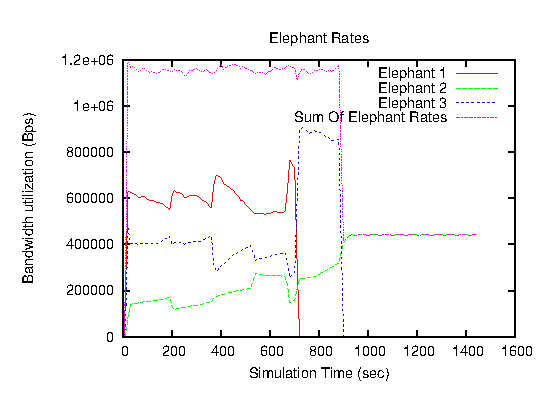
\includegraphics{elephant_bw.eps}
  \caption{Plot of the bandwidth utilization of each elephant, as well as the total bandwidth utilization of all elephants.}
  \label{fig:elephant_bw.eps}
\end{center}

\end{document}
